\section{矢量可以表示的东西}

许多物理和运动学对象——从一点到另一点的位移、作用在粒子上的力、刚体绕轴的有限旋转——都有方向和大小。 我们可以用矢量来表示这些属性\footnote{诸如“表示力的属性的矢量$\bb{F}$”之类的短语用来描述力的性质是精确的。 为了方便,我们可以将其简化为“表示力的矢量 $\bb{F}$”,甚至可以简化为“力$\bb{F}$”。 当上下文表述清晰时,简短的“$\bb{F}$”可能就足够了。},在这样做时,我们必须牢记两个基本点。

\begin{figure}[htbp]
	\centering
	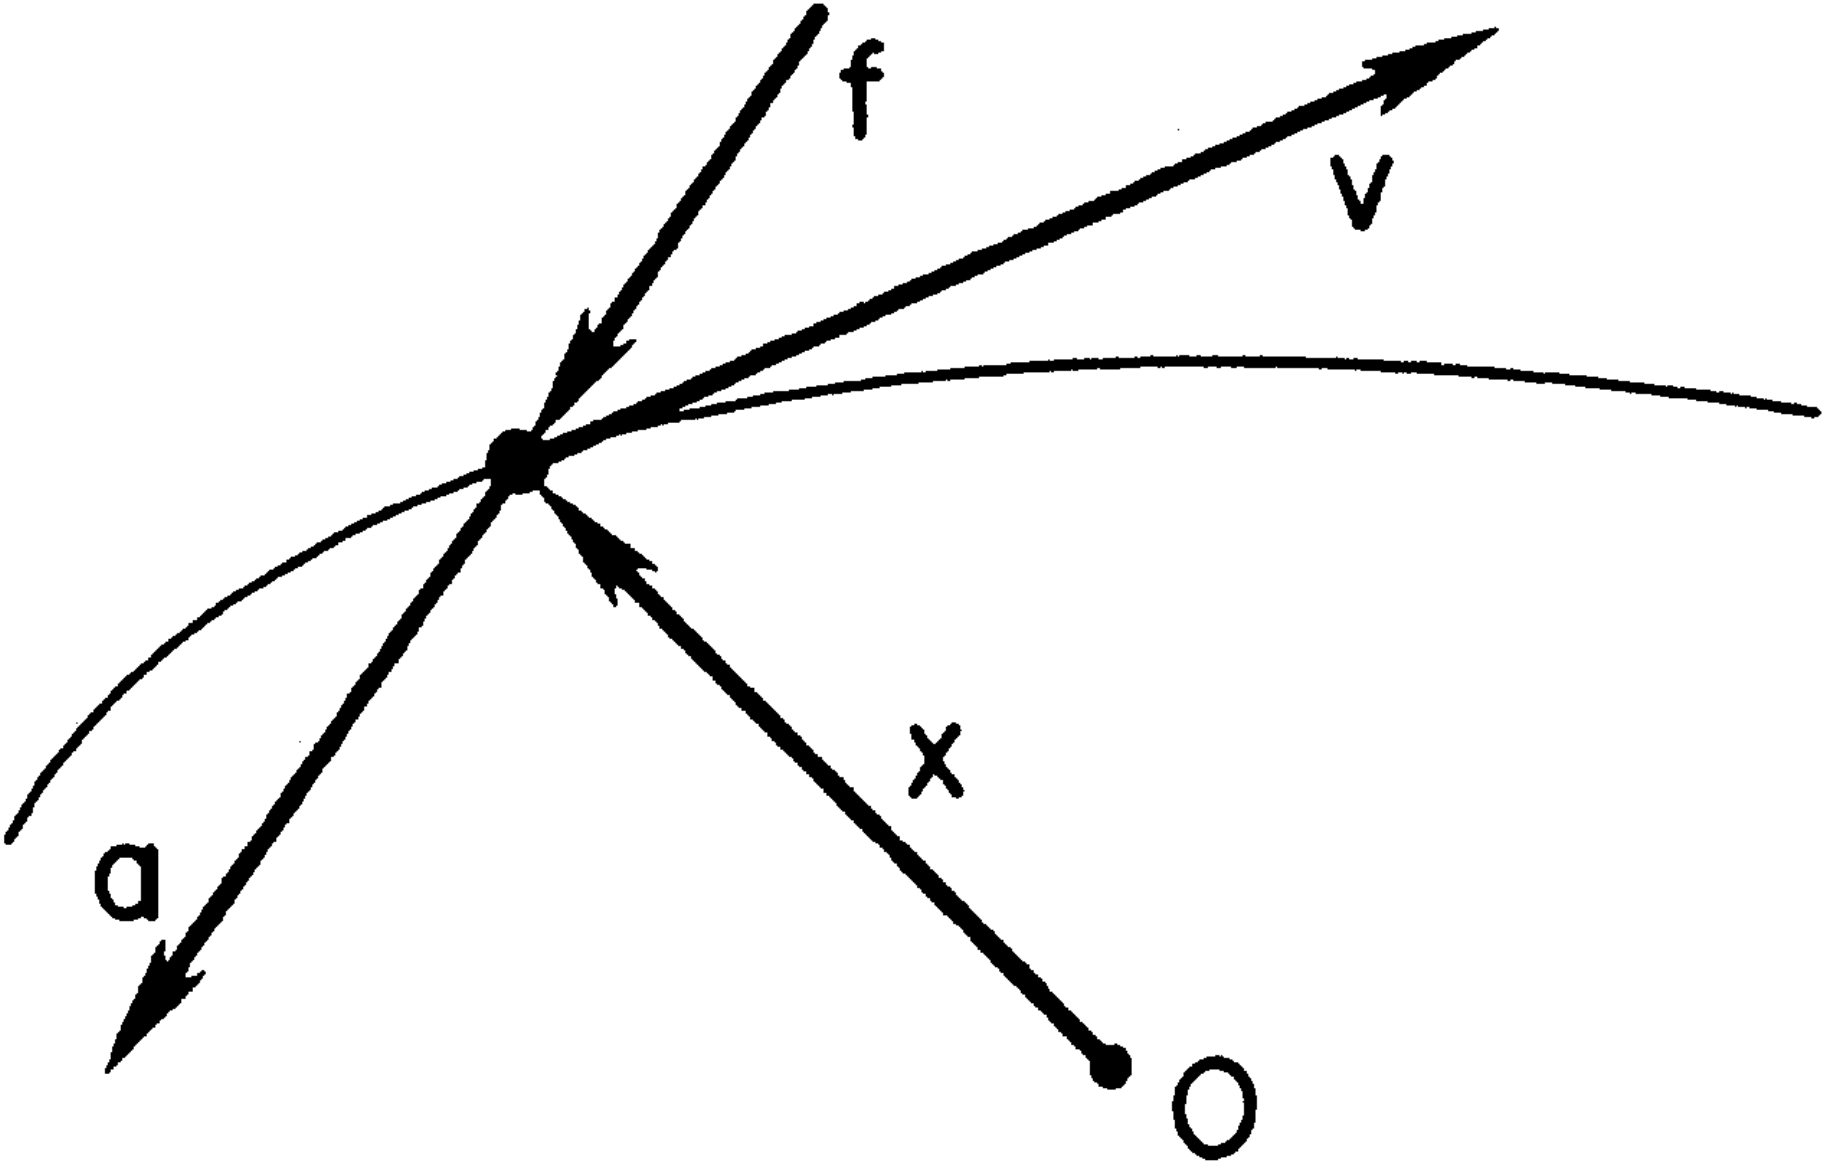
\includegraphics[width=0.4\textwidth]{./image/1.4.png}
	\caption{}
	\label{fig:1.4}
\end{figure}

重点1:\textbf{不同类型的对象由属于不同矢量空间的矢量表示。}否则,我们可以将力与位移混为一谈。不过,为了简洁明了,我们经常将不同类型的矢量放在同一张图片中,如图\eqref{fig:1.4}所示,它显示了在空中飞行的炮弹的位置$\bb{x}$、速度$\bb{v}$、加速度$\bb{a}$和作用其上的力$\bb{F}$。


重点2:\textbf{矢量加法不一定能反映物体的属性。}对于位移、力或速度,矢量加法有明显的物理含义;对于刚体围绕固定点的连续有限旋转,则没有。关于矢量加法,我们将在后文详述\footnote{物理学中,位移、力和速度的相加方式存在差异:位移遵循三角线法则,力在公共点处遵循平行四边形法则,而速度“像矢量相加”只是因为连续介质力学考虑了运动参考系这一假设。在相对论中,速度不相加。}。